\chapter{Considerações Preliminares}
\label{consideracoes}

Software livre/público já está consolidado como um tipo de software confiável 
devido ao nível de segurança proporcionado pelo seu uso, eliminação das mudanças
impostas pelo modelo proprietário, independência tecnológica, possibilidade de
auditabilidade além da gratuidade de suas licenças entre outras características.
%
Neste trabalho procuramos entender as dificuldades do governo em utilizar software
livre/público abordando o efeito de suas licenças e restrições de uso e como são 
tratado os direitos autorais desses softwares no Brasil.

Para investigar a hipótese levantada neste trabalho, a pesquisa bibliográfica 
apresentada estudou o processo de desenvolvimento utilizado pelo governo, também foi 
estudada a administração e suas teorias para entendermos a origem das metodologias
de desenvolvimento do governo e do software livre/público bem como o conceito de 
governança.

Com este trabalho foi possível notar a que a diferenciação das metodologias estão
na origem das mesmas tendo como base a teoria geral da administração, onde pude reparar
que a teoria humanística utilizada no desenvolvimento de software livre/público se
opõe a teoria de Taylor que tem suas bases nos processos e é utilizada pelo governo.

Para o desenvolvimento deste trabalho será utilizada a metodologia de pesquisa chamada
pesquisa-ação, onde primeiramente é feita uma pesquisa bibliográfica para entender
o problema para a partir desse ponto gerar uma ação. Entenda em detalhes na próxima sessão.

\section{Pesquisa-ação}

A pesquisa-ação ou action-research surgiu na década de 1940, no contexto de críticas ao uso
de procedimentos clássicos de ciências naturais na pesquisa social por razões de ordem prática 
(conhecimento teórico gerado teria pouca aplicabilidade na prática) ou ideológica (pesquisas estariam
sendo realizadas como uma forma de controle social)\cite{gil2010metodos}.

O pesquisador na pesquisa-ação
assume como premissa que processos sociais complexos, como a interação
entre organizações e seus sistemas de informação, são melhor investigados
quando se introduzem mudanças nestes processos e se observa os efeitos
destas mudanças. Outra premissa é que estes processos devem ser
investigados como uma entidade completa, não sendo possível extrair o objeto
de investigação do seu contexto. Desta forma, na pesquisa-ação busca-se avançar na teoria 
atuando na prática, o que é feito através de
ações no contexto de uma organização específica. O foco do pesquisador é na
compreensão do problema e das ações realizadas para solucioná-lo dentro de
um ambiente real particular e não na verificação de uma hipótese de caráter
geral num ambiente de laboratório~\cite{fuks2008suporte}.

\begin{figure}[htpb]
 \begin{center}
    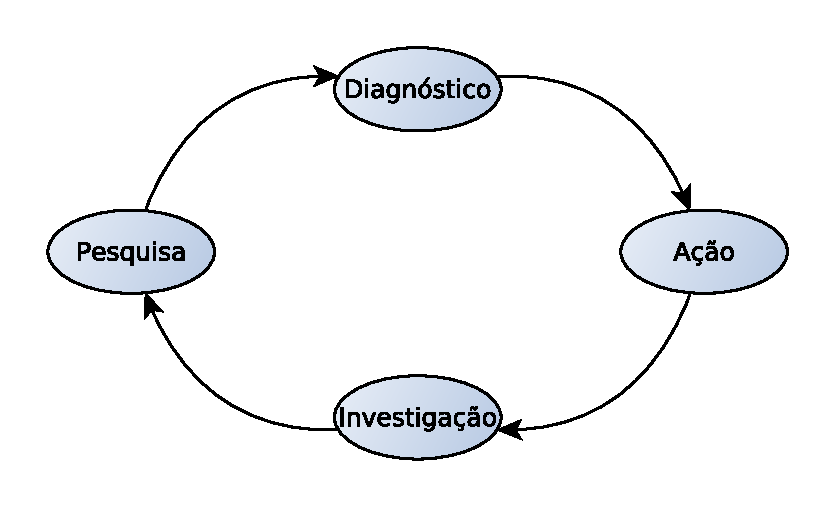
\includegraphics[width=.70\textwidth]{figuras/pesquisa-acao.eps}
 \end{center}
  \caption{Ciclo de desenvolvimento da pesquisa-ação}
  \label{fig:pesquisa-acao}
\end{figure}

Segundo Ana Paula~\cite{dos2012aplicaccao} "O pesquisador pode ter uma visão de \emph{insider}
ou \emph{outsider}, na realização de uma pesquisa-ação.
A visão de um \emph{insider} ocorre quando o pesquisador vivencia o problema e o traz para a pesquisa,
ou seja leva seus problemas para realizar a pesquisa, já a visão de outsider é quando a instituição
tem um problema e chama um pesquisador ou o pesquisador vai atrás de uma empresa ou cenário
real que tenha o problema". 

No caso desta pesquisa, estarei dentro de um contexto de 
desenvolvimento para o governo por participar do Projeto do Novo Portal do Software
Público, desta forma a pesquisa pode ser classificada como \emph{insider}.


\subsection{Abordagem Quantitativa versus Qualitativa}

As pesquisas, conforme as abordagens metodológicas que englobam, são classificadas em
dois grupos distintos – o quantitativo e o qualitativo. O primeiro obedece ao paradigma
clássico (positivismo) enquanto o outro segue o paradigma chamado alternativo~\cite{terence2006abordagem}.

\newpage
\begin{table}[htb]
\center
\footnotesize
\begin{tabular}{|p{4cm}|p{5cm}|p{5cm}|}
  \hline
   \textbf{} & \textbf{Pesquisa quantitativa}  & \textbf{Pesquisa qualitativa}\\
    \hline
   	Inferência & Dedutivo & Indutivo\\
   \hline    
    	Objetivo & Comprovação & Interpretação\\
   \hline
	Finalidade & Teste de teorias, predição, estabelecimento de fatos, e teste de hipóteses & Descrição e entendimento de realidades variadas, captura da vida cotidiana e perspectivas humanas\\
   \hline
	Realidade investigada & Objetiva & Subjetiva e complexa\\
   \hline
	Foco & Quantidade & Natureza do objeto\\
   \hline
	Amostra & Determinada por critério estatístico & Determinada por critérios diversos\\
   \hline
	Característica da amostra & Grande & Pequena\\
   \hline
	Característica do instrumento de coleta de dados & Questões objetivas, aplicações em um curto espaço de tempo & Questões abertas e flexíveis\\
   \hline
	Procedimentos & Isolamento de variáveis. Anônima aos participantes & Examina todo o contexto, interage com os participantes\\
   \hline
	Análise dos dados & Estatística e numérica & Interpretativa e descritiva. Ênfase na análise do conteúdo\\
   \hline
	Plano de pesquisa & Desenvolvido antes do estudo ser iniciado & Evolução de uma idéia como aprendizado\\
   \hline
	Resultados & Comprovação de hipóteses & Proposições e especulações\\
   \hline
	Confiabilidade e validade & Pode ser determinada dependendo do tempo e do recurso & Difícil determinação, dada a natureza subjetiva da pesquisa\\
   \hline
\end{tabular}
\caption{Características das abordagens qualitativa e quantitativa~\cite{terence2006abordagem}.}
\end{table}

Considerando as características apresentadas, a pesquisa desenvolvida neste trabalho
terá uma abordagem qualitativa por sua natureza indutiva, subjetiva e complexa, que será 
determinada por critérios diversos.

\section{Problema}

O Software Livre possui um mecanismo de produção colaborativo e dinâmico 
e possui uma organização composta por um conjunto de pessoas que usa e desenvolve 
um único software livre, contribuindo para uma base comum de código-fonte e 
conhecimento~\cite{reis2003caracterizacc}.

Este modelo típico do Software livre se diferencia em muitos aspectos com a forma
que o governo brasileiro desenvolve software, onde se estabelece um rígido processo.

Apesar disso, por fatores sociais e econômicos o governo brasileiro vem
criando políticas de incentivo a software livre, mas a dificuldade está em como
fazer a governança de dois mecanismos de gestão da produção de software antagônicos. 

\section{Hipótese}

As boas práticas de desenvolvimento a serem utilizadas em um projeto de software 
dependem do contexto, uma equipe que desenvolve software livre utiliza
meios diferentes para gerenciar o próprio projeto, que pode conter especificidades 
que impedem o uso de determinadas práticas impostas pelo governo federal para controle
do desenvolvimento de software. 

Dessa forma, com base no problema proposto, elaboramos a seguinte hipótese:

\begin{itemize}
\item Com algumas adaptações o processo do SISP pode se adequar
ao processo de desenvolvimento do software livre/público, a partir das boas práticas 
de colaboração dos mesmos.
\end{itemize}

Discutimos no Capítulo~\ref{software_livre} o tratamento que o governo
tem dado para o desenvolvimento de software livre/público mas ainda existem procedimentos
impostos pelo processo de desenvolvimento utilizado pelo governo, mostrados no Capítulo
\ref{governanca}, que não aproveitam o ecossistema de desenvolvimento de software livre/público.
%
A partir de boas práticas de colaboração com o software livre/público será possível
adaptar o processo de desenvolvimento PSW-SISP para suportar estes tipos de software e 
dessa forma dar oportunidade para que as comunidades de software livre possam desenvolver 
para o governo. 


\section{Resultados preliminares}

O foco deste trabalho é adequar a metodologia de desenvolvimento do governo com a
metodologia utilizada pelas grandes comunidades de software livre a partir de boas 
práticas utilizadas por essas comunidades.
Está em desenvolvimento um documento com boas práticas operacionais do novo portal 
do software público e sua primeira versão está disponível no repositório do projeto
\footnote{https://gitlab.com/softwarepublico/workflow}.

No documento apresentado como governança operacional do Novo Portal do Software Público
são destacadas as interações dos usuários nos ambientes e a partir desta interação é 
possível extrair boas práticas de desenvolvimento de software livre/público.

No documento o Novo Portal é dividido em ambientes onde os usuários podem ter diferentes 
tipos de interação. O primeiro ambiente, chamado ambiente de comunicação, estão contidas 
as listas de e-mails das comunidades, esta prática é muito adotada pelas comunidades
de desenvolvimento de software para abrir discussões técnicas e de negócio a respeito do 
software a ser desenvolvido.

O segundo ambiente é o chamado ambiente de colaboração, neste ambiente serão disponibilizados
os códigos-fonte dos software que estão no portal e faz uso das boas práticas adotadas pelas 
comunidades de desenvolvimento de software para versionamento e controle do desenvolvimento.

O terceiro ambiente é uma rede social para os usuários do portal, onde será possível participar
das comunidades dos softwares, ler notícias, baixar os softwares entre outras funcionalidades.   




\section{Próximos passos}

Para alcançar os objetivos deste trabalho, serão realizadas as seguinte macro-atividades
na segunda etapa deste trabalho. Seguindo a metodologia proposta utilizarei os conhecimentos
adquiridos na pesquisa desta etapa do trabalho para apresentar uma ação para resolver o 
problema segundo a tabela~\ref{cronograma}.


\begin{table}[htb]
\center
\footnotesize
\begin{tabular}{|p{8cm}|p{3cm}|p{3cm}|}
  \hline
   \textbf{Atividade} & \textbf{Início} & \textbf{Fim}\\
    \hline
	Aprofundar estudo de metodologia de desenvolvimento do governo & 01/02/2015 & 01/03/2015\\
    \hline
	Aprofundar estudo de metodologia de desenvolvimento software livre/público & 01/02/2015 & 01/03/2015\\
    \hline
        Caracterizar os processos de desenvolvimento buscando pontos de intersecção & 02/03/2015 & 15/03/2015\\
    \hline
	Coletar experiência e boas práticas dos usuários das metodologias & 16/03/2015 & 01/04/2015\\
    \hline
	Analisar dados coletados & 02/04/2015 & 15/04/2015\\
    \hline 
	Discutir resultados encontrados & 16/04/2015 & 01/05/2015\\
    \hline
	Montar governança adequada com base nos resultados & 02/05/2015 & 01/06/2015\\
    \hline
	Discutir governança proposta & 02/06/2015 & 20/06/2015\\
    \hline
	Entrega do TCC2 & 20/06/2015 & 30/06/2015\\
    \hline
\end{tabular}
\caption{Cronograma para o TCC2}
\label{cronograma}
\end{table}

As primeiras atividades de aprofundamento de estudo das metodologias serão 
necessárias que ocorram paralelamente para que já seja buscada uma comparação 
entre as mesmas e estas atividades darão subsídios para que sejam caracterizados 
os dois processos de desenvolvimento.
%
Coletar experiência dos usuários será uma maneira de observar as boas práticas de cada 
metodologia e com a análise das experiência poderei distinguir o que fica e o que 
é necessário que seja repensado em cada processo.
%
A metodologia proposta será montada a partir dessas experiências e estudos relacionados
trazendo embasamento para a metodologia proposta. 
